\documentclass[a4paper, 12pt]{article}
\usepackage[left=1.5cm, right=1.5cm, top=1.5cm, bottom=2.5cm]{geometry}
\usepackage[utf8]{inputenc}
\usepackage[russian]{babel}
\usepackage{verbatim}
\usepackage{graphicx}
\usepackage{listingsutf8}
\usepackage{color}
\usepackage{ulem}
\usepackage{amsmath}
\usepackage{array}
\usepackage{amssymb, latexsym, amsmath, textcomp}
\usepackage{indentfirst}
\usepackage{cmap}
\usepackage{graphics}
\usepackage{listings}
\usepackage{enumerate}
\usepackage{wrapfig}

\lstset{
basicstyle=\footnotesize,
breaklines=true,
numbers=left,
extendedchars=\true,
numbersep=7pt,
caption=\lstname,
frame=single,
inputencoding=utf8,
showstringspaces=\false
}

\newenvironment{enumerate*}%
  {\begin{enumerate}%
    \setlength{\itemsep}{1pt}%
    \setlength{\parskip}{1pt}}%
  {\end{enumerate}}
\newenvironment{itemize*}%
  {\begin{itemize}%
    \setlength{\itemsep}{1pt}%
    \setlength{\parskip}{1pt}}%
  {\end{itemize}}

%------------------------------------------------------------------------------------------------------------------------------
%------------------------------------------------------------------------------------------------------------------------------
\begin{document}

\begin{titlepage}
\begin{center}
{Санкт-Петербургский национальный исследовательский университет информационных технологий, механики и оптики}

Кафедра вычислительной техники
\end{center}
\vspace{50mm}
\begin{center}
\begin{tabular}{c}
\Huge{\textbf{Отчёт}}\\
\Large{\textbf{по лабораторной работе №4}}\\
\Large{\textbf{дисциплины <<Программирование интернет-приложений>>}}\\
\Large{\textbf{Вариант №483}}\\[2mm]
\end{tabular}
\end{center}
\vspace{85mm}
\begin{flushright}
\begin{tabular}{l}
Выполнили:\\
студенты гр. P3211\\
Ефремов Р.В.,\\
Синицкий Д.П.\\
Преподаватели:\\
Цопа Е.А.\\
Письмак А.Е.\\
\\
\end{tabular}
\end{flushright}
\vspace{15mm}
\begin{center}
Санкт-Петербург - 2017 г.
\end{center}
\end{titlepage}
\newpage

\section{Текст задания}

Переписать приложение из предыдущей лабораторной работы с использованием следующих технологий:

\begin{itemize*}
\item Уровень back-end должен быть основан на Java EE (необходимо использовать EJB).
\item Уровень front-end должен быть построен на Angular 2 (Angular 3) с использованием обычных полей ввода HTML
\item Взаимодействие между уровнями back-end и front-end должно быть организовано посредством REST API.
\end{itemize*}

\begin{wrapfigure}{r}{0.2\textwidth}
\begin{center}
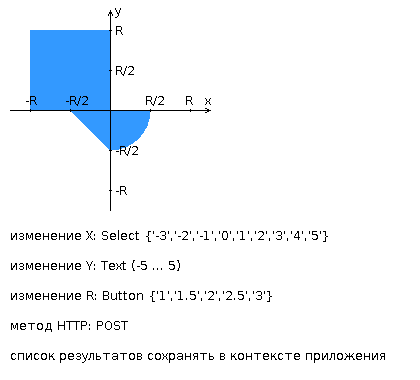
\includegraphics[width=0.2\textwidth]{img/areas.png}
\end{center}
\end{wrapfigure}


Приложение по-прежнему должно включать в себя 2 страницы - стартовую и основную страницу приложения. Обе страницы приложения должны быть адаптированы для отображения в 3 режимах:
\begin{itemize*}
\item ''Десктопный'' - для устройств, ширина экрана которых равна или превышает 1217 пикселей.
\item ''Планшетный'' - для устройств, ширина экрана которых равна или превышает 660, но меньше 1217 пикселей.
\item ''Мобильный''- для устройств, ширина экрана которых меньше 660 пикселей.
\end{itemize*}

\paragraph{Стартовая страница должна содержать следующие элементы:}
\begin{itemize*}
\item ''Шапку'', содержащую ФИО студента, номер группы и номер варианта.
\item Форму для ввода логина и пароля. Информация о зарегистрированных в системе пользователях должна храниться в отдельной таблице БД (пароль должен храниться в виде хэш-суммы). Доступ неавторизованных пользователей к основной странице приложения должен быть запрещён.

\end{itemize*}

\paragraph{Основная страница приложения должна содержать следующие элементы:}
\begin{itemize*}
\item Набор полей ввода для задания координат точки и радиуса области в соответствии с вариантом задания: Select {'-4','-3','-2','-1','0','1','2','3','4'} для координаты по оси X, Text (-5 ... 5) для координаты по оси Y, и Select {'-4','-3','-2','-1','0','1','2','3','4'} для задания радиуса области. Если поле ввода допускает ввод заведомо некорректных данных (таких, например, как буквы в координатах точки или отрицательный радиус), то приложение должно осуществлять их валидацию.
\item Динамически обновляемую картинку, изображающую область на координатной плоскости в соответствии с номером варианта и точки, координаты которых были заданы пользователем. Клик по картинке должен инициировать сценарий, осуществляющий определение координат новой точки и отправку их на сервер для проверки её попадания в область. Цвет точек должен зависить от факта попадания / непопадания в область. Смена радиуса также должна инициировать перерисовку картинки.
\item Таблицу со списком результатов предыдущих проверок.
\item Кнопку, по которой аутентифицированный пользователь может закрыть свою сессию и вернуться на стартовую страницу приложения.
\end{itemize*}




\paragraph{Дополнительные требования к приложению:}
\begin{itemize*}
\item Все результаты проверки должны сохраняться в базе данных под управлением СУБД PostgreSQL.
\item Для доступа к БД необходимо использовать JPA.
\end{itemize*}

\newpage

\section{Код}

\lstinputlisting[language=Java]{../src/Application.java}
\lstinputlisting[language=Java]{../src/ejbs/ManagerBean.java}

\lstinputlisting[language=Java]{../../iadlab-front-end/src/app/app.routes.ts}
\lstinputlisting[language=HTML]{../../iadlab-front-end/src/app/auth/register/register.component.html}
\lstinputlisting[language=Java]{../../iadlab-front-end/src/app/auth/register/register.component.ts}
\lstinputlisting[language=HTML]{../../iadlab-front-end/src/app/main/canvas/canvas.component.html}
\lstinputlisting[language=Java]{../../iadlab-front-end/src/app/main/canvas/canvas.component.ts}
\lstinputlisting[language=Java]{../../iadlab-front-end/src/app/point.service.ts}
\lstinputlisting[language=Java]{../../iadlab-front-end/src/app/user.service.ts}

\section{Выводы по работе}
В ходе подготовки к выполнению данной лабораторной работы были изучены основы создания веб-приложений в соответствии со спецификацией Enterprise Java Beans, 
а именно создание бинов, контекст существования, прицнипы Dependency Injection и Inverse Of Control. Также для реализации REST API были использованы средства JAX-RS API.    

В реализации фронтенд-части был использован фреймворк Angular, использованы его средства для создания компонентов, соответсвующих им template HTML страниц, 
взаимодействия компонентов между собой и сервисами.
 
С использованием полученных знаний в соответствии с заданием было реализовано и развернуто на сервере Glassfish веб-приложение. 

\end{document}
